%\subsection{Récupération de l'image du corps humain}
%SDK de la kinect avec skelette
%\subsection{Préparation de l'image}
%suppression du bruit et diminution du nombre de point -> pcl
%\subsection{Segmentation du corps humain}
%distance geodesic avec dikjstra -> pb nombre de voisin
%superpixel
%\subsection{Reconnaissance des parties du corps}
%descripteur D2 avec model 3D
%FPFH
%\subsection{Appariement d'un model 3D}
%scale à partir d'une bounding box
%ICP
%moment d'inertie
%\subsection{Résultat des expérimentations}
%montrer plusieurs images de la segmentation et montrer ce qui ne convient pas
%dire que les méthode utilisé seront utilisé dans la suite du projet 
\subsection{Objectif}
%on cherche a ne pas utiliser la kinect
Cette première application a plusieurs objectifs. Dans un premier temps, nous souhaitons réaliser 
une segmentation sans utiliser les outils fournis pas la Kinect dans le but d'obtenir une méthode plus
précise ou tout du moins permettant d'améliorer une partie du procédé de segmentation. Comme nous l'avons vu dans 
l'état de l'art, les méthodes utilisées par la Kinect ont évolué et sont devenu plus stable et plus précise.
Le second objectif et de remplacer un nuage de point représentant un membre par un modèle 3D de ce même membre
mais ayant une forme différente. Cette première partie du stage me permet surtout d'aborder des concepts qui me 
serviront dans la second application qui est le but premier de ce stage.

\subsection{Délimitation du corps humain et minimisation de la quantité de donnée}
%prétraitement
%utilisation voxel pour réduire le nombre de point
%utilisation d'outils pour supprimer les outlier
%utilisation de threshold
%suppression d'objet à la main
%utilisateur peut les modifier lui meme
%finalement utilisation de la Kinect pour la delimitation
Durant cette première phase nous travaillons sur un nuage de point et non sur les informations de l'image de profondeur.
Comme nous l'avons dit précédemment, l'ensemble des informations n'est pas pértinente pour les traitements que nous souhaitons
réaliser. Dans cette première application il nous faut dabord supprimer l'ensemble des informations qui ne se rapporte pas 
au corps humain. La première solution que j'ai utilisé et qui était la plus simple a été de mettre deux seuil afin de 
supprimer les informations qui sont au-dessus d'un certain seuil ainsi que les informations qui sont en-dessous d'un second
seuil. Ces seuils sont les distances, en mètre, dans lequel l'utilisateur doit se trouver. Cette méthode est utilisé dans 
l'application ReconstructMe\footnote{http://reconstructme.net} qui est une application permettant de construire un modèle
3D complet à partir de données fournit par plusieurs images provenant d'une caméra 3D. Comme pour cette application, j'ai
décidé de laisser la possibilité à l'utilisateur de changer les seuils en fonction de sont besoin.\\

%TODO mettre une image délimitant le corps humain avec des seuils
\begin{figure}[!ht]
  \begin{center}
    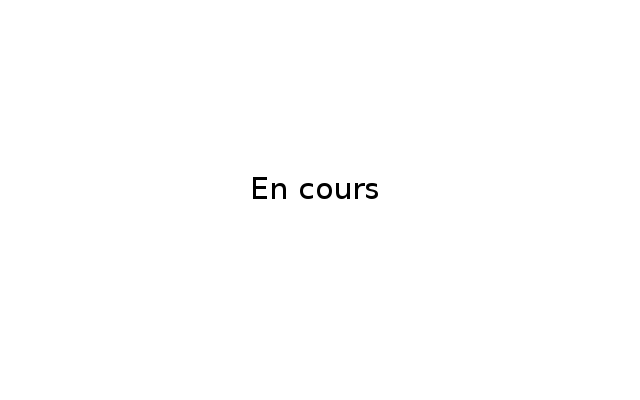
\includegraphics[width=5cm]{image/wait.png}
    \caption{Résultat d'une segmentation par seuillage}
    \label{fig:seuillage}
  \end{center}
\end{figure}

Nous pouvons voir sur la Fig. \ref{fig:seuillage} que le seuil permet effectivement de supprimer beaucoup d'information
correspondant à l'environnement, mais qu'il reste beaucoup de bruit du à la qualité de l'acquisition de la caméra. La librairie
PCL\cite{PCL} nous fournit beaucoup d'outil pour ce genre de problèmatique. Il y a une classe appelé StatisticalOutlierRemoval
qui permet de supprimer les points supposé être du bruit. Pour cela cette classe calcul la distance moyenne d'un point avec son
voisinnage et si cette moyenne est trop élevé, elle supprime le point en question.\\

%TODO mettre une image délimitant le corps humain avec des seuils et avec la suppression du bruit
\begin{figure}[!ht]
  \begin{center}
    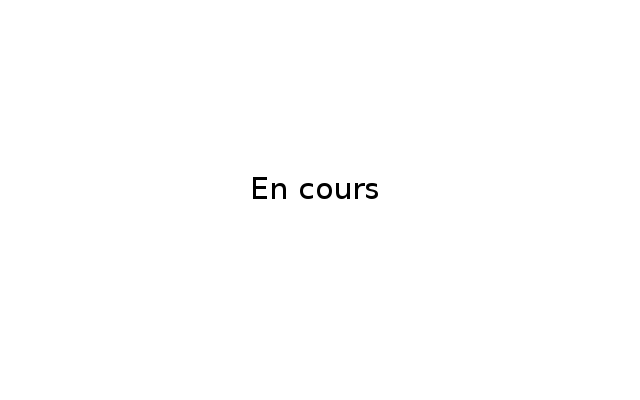
\includegraphics[width=5cm]{image/wait.png}
    \caption{Résultat d'une segmentation par seuillage avec suppression du bruit}
    \label{fig:seuillageOutlier}
  \end{center}
\end{figure}

Pour la suite des traitements que nous souhaitons réalisé, il est préférable d'avoir un minimum d'information et de ne garder
que ce qui est pertinant. Le corps humain que nous avons réussi à délimité comporte encore beaucoup trop de données. Le nombre
de point fournit par la Kinect est très important et très concentré, il est possible de supprimer des points qui sont trop 
proche les uns les autres. La encore PCL\cite{PCL} peut nous aider avec la classe VoxelGrid. Cette classe crée une grille de
voxel sur le nuage de point dont la taille est définit par l'utilisateur. L'ensemble des points à l'intérieur d'un voxel sont 
approximé en un point qui correspond au centroïde du voxel. Grâce à l'ensemble de ces traitements nous ne gardons que l'information 
essentiel à nos traitement.

\subsection{Calcule de la distance géodésique}
Ma première idée pour segmenter le corps humain est d'utiliser la distance géodesique. Y. Liu et al\cite{GIF} montre que la distance
géodesique pour une même personne quelque soit sa posture est toujours la même pour les points de ces membres. Le seul problème 
est que plusieurs membres ont la même distance géodésique, on ne peut donc pas associer un membre à une distance directement.
Cependant, s'il est possible de seuiller le corps et d'en calculer des descripteurs, nous pourrons déterminer quel nuage de point
correspond à quel membre.\\

Avant de calculer la distance géodésique du corps humain, nous avons besoin de créer un maillage sur le nuage de point. Pour cela
j'ai repris le principe utilisé pour le descripteur FPFH\cite{FPFH} pour la sélection des voisins. Dans un premier temps je calcule
la distance euclidienne de chacun des points du nuage de point avec tous les autres. Pour la création du voisinage je considère non
seulement le nombre maximum de point à prendre en compte, mais aussi la distance maximum d'un point avec les autres. Nous avons eu
plusieurs problème lorsque nous n'avions pas mis la second condition, car lorsque la main de l'utilisateur était trop proche de sa 
jambe certain point de la main avait des voisins dans la jambe.\\

%TODO voir si on met des exemples de maillage defectueux 

A cette étape de l'algorithme nous avons donc un maillage et les distances euclidiennes de chaque point avec son voisinnage. Pour calculer
la distance géodésique du centroïde du nage de point avec chaque point nous allons utilisé l'algorithme de Dijkstra\cite{dijkstra}.
Il faut donc trouver le plus court chemin du centroïde jusqu'au point dont on veut calculer la distance géodésique en passant par le
maillage que nous avons construit précédemment. A chaque fois qu'un point est ajouté au chemin emprunté par l'algorithme il faut 
additionner la distance euclidienne entre ce point et le précédent pour obtenir un résultat final correspondant à la distance 
géodésique.\\

%TODO ajout d'une image d'un corps humain avec un chemin ?
\begin{figure}[!ht]
  \begin{center}
    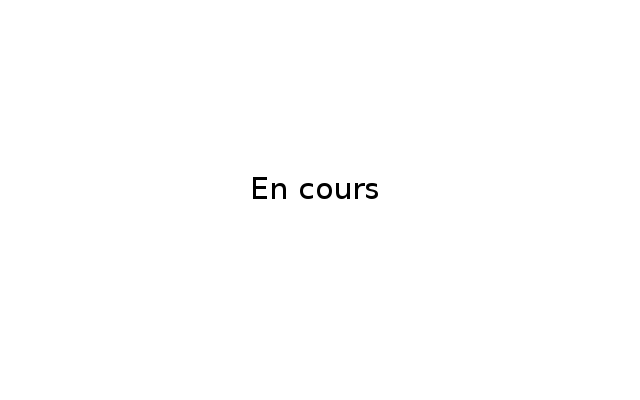
\includegraphics[width=5cm]{image/wait.png}
    \caption{Exemplre de chemin parcouru par l'algorithme de calcul de la distance géodésique pour un point}
    \label{fig:cheminGeodesique}
  \end{center}
\end{figure}

%TODO refaire les images
\begin{figure}[!ht]
  \begin{center}
    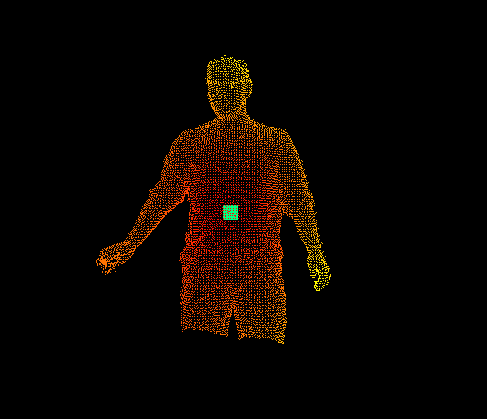
\includegraphics[width=6.5cm]{image/geodesic1.PNG}
    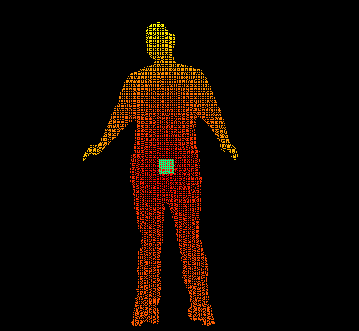
\includegraphics[width=6cm]{image/geodesic2.PNG}
    \caption{Résultat du calcul de la distance géodésique sur l'ensemble du nuage de point. Le point vert correspond au centroïde du
    nuage de point. Plus la couleur des points est proche de rouge, plus les points sont proches du centroïde.}
    \label{fig:cheminGeodesique}
  \end{center}
\end{figure}

 
\subsection{Calcule de descripteurs}
%d2
\subsection{SDK de la Kinect}
%récuperation du corps de la personne depuis une image kinect -> a partir des info de la kinect -> le mettre plutot dans les travaux réalisé
%labelisation en fonction de la distance du point avec le joint
\subsection{Positionnement}
%icp, fpfh
%dire qu'il n'est pas possible d'utiliser la distance geodesic pour le positionnement a cause du temps et qu'on ne peut calculer la distance geodesic
%sur le mesh de remplacement
